\chapter{Crystallization of the crust of a non-accreting neutron star}

% crystallization temperature is a lower estimate for the temperature at which 
%   nuclear reactions fall out of equilibrium (see ic sh paper)

\minitoc\newpage

\section{Model of the crust at finite temperature}

% in this study, no proton drip nor pasta phases are considered in the
%   free neutron regime. one can assume that proton drip does not occur in the
%   range of temperature considered here. Pasta phases are difficult to account
%   for within the mcp treatment

\subsection{One-component Coulomb plasma approximation}

At zero temperature, WS cells are supposed to be identical, thus the OCP  
(single-nucleus) approximation~\cite{Baus1980}, which considers a unique 
nucleus $(A,Z)$ for a given thermodynamic condition of pressure and temperature 
$(P,T)$, is exact. Let us recall that the equilibrium composition is 
determined by minimizing the Gibbs free energy per nucleon at fixed
pressure~\cite{Fantina2020} 
(or equivalently the free energy density at fixed baryon
density~\cite{Lattimer1991,Gulminelli2015,Carreau2019}).
At finite temperature in the OCP approximation, the expected distribution of 
nuclei is replaced by the equilibrium nucleus obtained from the minimization of 
the relevant thermodynamic potential.
The physical properties of the OCP are fully characterized by the so-called 
dimensionless Coulomb coupling parameter,
%
\begin{equation}
  \Gamma = \frac{Ze^2}{a_N k_B T},\label{eq:gamma}
\end{equation}
%
where $a_N=(4\pi n_N/3)^{-1/3}$ is the ion-sphere radius, $n_N=1/V_{WS}$ being 
the ion density.
More precisely, $\Gamma$ allows to quantify the nonideality of the system, that
is the importance of the many-body interactions in the OCP. The lower the
temperature, the more coupled are the ions. The crystallization of the OCP into 
a lattice is observed at $T=T_m$, corresponding to 
$\Gamma = \Gamma_m \approx 175$.

The total free energy per ion in the crust is given by
%
\begin{equation}
  F = F_{i,e} + F_g + F_e,\label{eq:fperion}
\end{equation}
%
where $F_{i,e}$ is the ion free energy in the e-cluster representation 
(see~\ref{subsec:nucenergy}), $F_g$ is the neutron gas free energy, and $F_e$ 
is the electron gas free energy, given by~\cite{Haensel2007}
%
\begin{equation}
  \mathcal{F}_e = \frac{F_e}{V_{WS}} = \varepsilon_e -
  \frac{P_r}{6}t_r^2x_r\gamma_r,\label{eq:fel}
\end{equation}
%
with $t_r = T/(m_e c^2)$. The expressions of the energy density 
$\varepsilon_e$, relativistic unit of the electron pressure $P_r$, relativity
parameter $x_r$, and $\gamma_r$ are given in~\ref{subsubsec:elgas}. It should
be stressed that Eq.~(\ref{eq:fel}) is obtained by employing a Sommerfeld
expansion in the limit $t_r \ll \gamma_r - 1$.
Let us notice that in the regime of the outer crust, neutrons are still bound
to the nuclei, thus $F_g=0$ MeV, and consequently $F_{i,e}$ coincides with the 
ion free energy in the r-cluster representation $F_i$.
The ion free energy reads
%
\begin{equation}
  F_{i,e} = M_{i,e} c^2 + F_i^{\text{id}} + F_i^{\text{int}},\label{eq:fie}
\end{equation}
%
where the ion mass in e-cluster representation $M_{i,e}$ has been introduced.
In Eq.~(\ref{eq:fie}), $F_i^{\text{id}}$ represents the ideal contribution to
the ion free energy, that is the noninteracting part, and $F_i^{\text{int}}$
the interacting part.

In the following, we give the expressions associated to the ideal and 
interacting contributions to the ion free energy which differ according to the 
phase of matter, either solid or liquid. In the free neutron regime, the 
finite-size contribution is included and is common to both phases. The latter 
is derived from the application of Gauss theorem,
%
\begin{equation}
  E_{fs} = \frac{2n_p}{n_0(1-I)}\frac{e^2}{r_0}\frac{Z^2}{A^{1/3}},
\end{equation}
%
where $r_0=(4\pi n_0/3)^{-1/3}$ is related to the average density of the
cluster $n_0$.
The modeling of $M_{i,e}$ as well as of the neutron gas free energy $F_g$ is 
presented in detail in~\ref{subsec:freeenfunctional}. 

\subsubsection{OCP in a liquid phase}

Above the crystallization temperature, $T > T_m$, the OCP is in a liquid phase.
In the Coulomb liquid, each ion can move freely within the volume of the WS 
cell in which it is confined. This translational center-of-mass motion is
accounted for in the noninteracting part of the ion free energy, which
therefore reads~\cite{Haensel2007}
%
\begin{equation}
  F_i^{\text{id}} = k_B T 
  \left[\ln\left(\frac{n_N\lambda^3}{g_s}\right) - 1\right]\label{eq:fliqid},
\end{equation}
%
where $g_s$ is the spin degeneracy, which we take $g_s=1$ for nuclei whose
ground-state angular momentum is unknown, and $\lambda$ is the de Broglie
wavelength of the component given by
%
\begin{equation}
  \lambda = \sqrt{\frac{2\pi(\hbar c)^2}{M_{i,e}c^2 k_B T}}.
\end{equation}
%

The interacting part of the ion free energy can be decomposed
as~\cite{Fantina2020}
%
\begin{equation}
  F_i^{\text{int}} = F_{ii,\text{liq}} +
  F_{ie,\text{liq}}^{\text{pol}}\label{eq:fiintliq}
\end{equation}
%
Analytical formulae have been derived for these two terms 
in~\cite{Potekhin2000}.
In the present study, we find that the importance of the correction
associated to electron polarization effects, 
$F_{ie,\text{liq}}^{\text{pol}}$ (Eq.~(19) of~\cite{Potekhin2000}), is very 
small in the density and temperature regime of interest, and is therefore 
neglected. The only significant effect of the latter correction is to change 
the crystallization temperature of $40-50\%$ around $P\approx 1.25\times 
10^{-4}$ MeV/fm$^3$, where the composition changes drastically due to 
shell structure~\cite{Fantina2020}.
For the total Coulomb contribution, we employ the parametrization 
proposed in~\cite{Potekhin2000}: 
%
\begin{eqnarray}
  \frac{F_{ii,\text{liq}}}{k_B T} 
  &=& A_1\left[\sqrt{\Gamma(A_2+\Gamma)} - A_2\ln\left(\sqrt{\Gamma/A_2} 
+ \sqrt{1+\frac{\Gamma}{A_2}}\right)\right]\notag\\
  &&+ 2A_3\left(\sqrt{\Gamma} - \arctan\sqrt{\Gamma}\right) 
  + B_1\left[\Gamma-B_2\ln\left(1+\frac{\Gamma}{B_1}\right)\right]\notag\\
  &&+ \frac{B_3}{2}\ln\left(1+\frac{\Gamma^2}{B_4}\right),
\end{eqnarray}
%
with $A_1=-0.9070$, $A_2=0.62954$, $A_3=-\sqrt{3}/2-A_1/\sqrt{A_2}$,
$B_1=4.56\times 10^{-3}$, $B_2=211.6$, $B_3=-10^{-4}$, and $B_4=4.62\times
10^{-3}$. Let us notice that the latter parametrization 
solely depends on the Coulomb coupling parameter $\Gamma$, 
Eq.~(\ref{eq:gamma}), and that $F_{ii,\text{liq}}$ vanishes at high 
temperature.

\subsubsection{OCP in a solid phase}

Once the crystallization temperature $T_m$ is reached, we assume that the OCP 
crystallizes into a perfect body-centered cubic lattice~\cite{Chamel2016}, as
in the zero temperature case studied in Chapter 1. In the solid OCP, ions are
able to oscillate near their equilibrium positions. Hence, the ideal 
part of the ion free energy accounting for the translational motion in the 
liquid OCP, $F_{i}^{\text{id}}$, is replaced by the zero-point motion energy, 
$E_{zp}$, Eq.~(\ref{eq:ezp}). The ion free energy in the e-cluster
representation is therefore rewritten as
%
\begin{equation}
  F_{i,e,\text{sol}} = M_{i,e}c^2 + E_{zp} + F_{ii,\text{sol}} +
  F_{ie,\text{sol}}^{\text{pol}},
\end{equation}
%
where $F_{ie,\text{sol}}^{\text{pol}}$ corresponds to the polarization
correction in the solid phase~\cite{Potekhin2000}, which is neglected here, and
$F_{ii,\text{sol}}$ is the Coulomb interaction term that can be decomposed as
%
\begin{equation}
  F_{ii,\text{sol}} = E_L + F_{\text{th}} + F_{\text{ah}} - k_B
  T\ln(g_s).\label{eq:fiisol}
\end{equation}
%
In the latter expression, $E_L$ represents the temperature-independent static 
lattice term, given by Eq.~(\ref{eq:eL}). The last term in~\ref{eq:fiisol} is
the spin entropy. As previously, we fix $g_s=1$ for nuclei whose spin 
degeneracy is unknown, yet the inclusion of this term has no effect on the 
determination of the crystallization temperature because it is the same for 
both liquid and solid OCP.

As for total Coulomb contribution in the liquid phase, the thermal
contribution due to the ion vibrations around their equilibrium position in the 
harmonic approximation and the anharmonic correction have been analytically
fitted by Baiko \textit{et al.}~\cite{Baiko2001} and Potekhin \&
Chabrier~\cite{Potekhin2010}, respectively. 
The expression employed for the thermal contribution reads~\cite{Baiko2001}
%
\begin{equation}
  \frac{F_{\text{th}}}{k_B T} = \sum_{n=1}^3\ln\left(1
    -\text{e}^{-\alpha_n\theta}\right) 
  - \frac{A(\theta)}{B(\theta)},
\end{equation}
%
where $\theta \equiv \hbar\omega_p/(k_B T)$, $\omega_p$ being the ion plasma
frequency, Eq.~(\ref{eq:omegap}), and
%
\begin{equation}
  A(\theta) = \sum_{n=0}^{8}a_n\theta^n,
\end{equation}
%
\begin{equation}
  B(\theta) = \sum_{n=0}^{7}b_n\theta^n 
  + \alpha_6 a_6 \theta^9 
  + \alpha_8 a_8 \theta^{11},
\end{equation}
%
with $\alpha_n$, $a_n$, and $b_n$ numerical constants (see Table II
in~\cite{Baiko2001}).
The analytical expression of the anharmonic correction used in our study
is~\cite{Potekhin2010}

\begin{equation}
  F_{\text{ah}} =
  F_{\text{ah}}^{(0)}\text{e}^{-c_1\theta^2} 
  - k_B T d_1\frac{\theta^2}{\Gamma},\label{eq:ah}
\end{equation}
%
where
%
\begin{equation}
  F_{\text{ah}}^{(0)} = k_B T\sum_{n \geq 1}\frac{f_n}{n\Gamma^n}
\end{equation}
%
with $c_1$, $d_1$, and $f_n$ numerical constants. One should stress that
the latter expression is modified with respect to that proposed by Farouki \&
Hamaguchi, $F_{\text{ah}}^{(0)}$, based on numerical simulations of 
the solid OCP for $170 \leq \Gamma \leq 2000$~\cite{Farouki1993}, so as to
reproduce the zero-temperature and classical limits.

\subsubsection{Crystallization of a OCP}

As in previous works~\cite{Fantina2020,Carreau2019,Carreau2020}, we compute 
the crystallization temperature within the OCP approximation, which is 
simple and not costly from the numerical point of view. An additional reason is
that the ion distribution  could be frozen at some temperature $T_f > T_m$ 
considering the present uncertainties on timescales relative to NS 
cooling~\cite{Goriely2011}.

\begin{figure}[!t]
  \begin{center}
    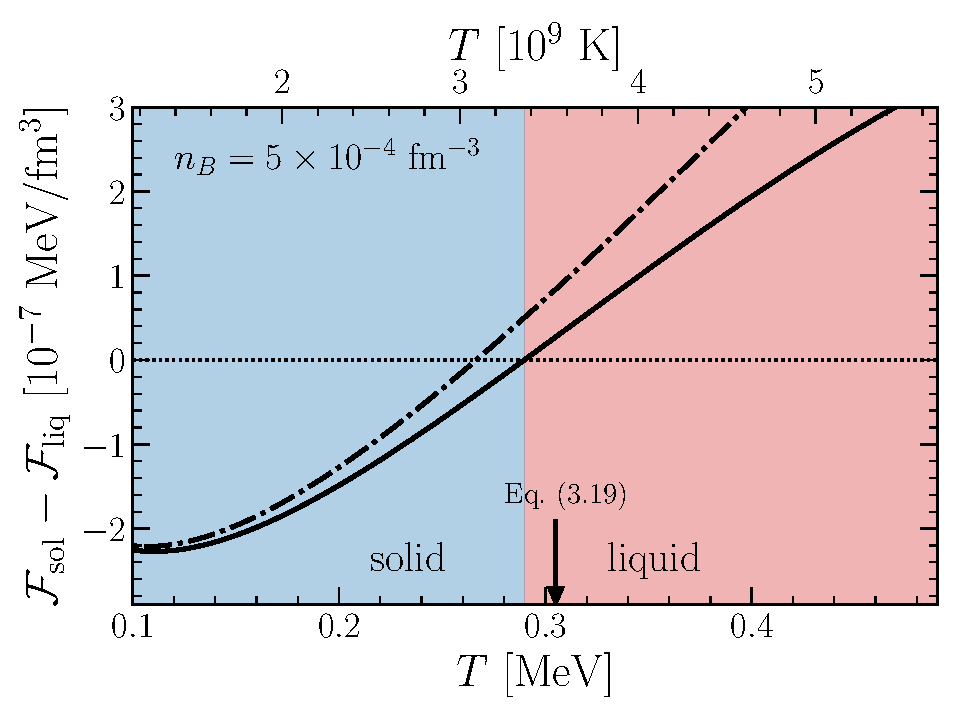
\includegraphics[width=0.9\linewidth]{figures/fliqsol.pdf}
  \end{center}
  \caption[Free energy density difference between liquid and solid phases
  versus temperature]{Variation with temperature $T$ of the free energy density
  difference between liquid and solid phases
$\mathcal{F}_{\text{sol}}-\mathcal{F}_{\text{liq}}$ for the optimal composition
$\bm{\theta_{\text{liq}}}$ at $n_B=5\times 10^{-4}$ fm$^{-3}$ (free neutron 
regime) with (solid line) and without (dashdotted line) the anharmonic
contribution, Eq.~(\ref{eq:ah}), to the free energy in the solid 
phase, using BSk24 CLDM. The crystallization temperature obtained from 
Eq.~(\ref{eq:tmapprox}) is also indicated.}\label{fig:fliqsol}
\end{figure}

The condition of crystallization of a OCP with associated composition 
$\bm{\theta}$ is 
%
\begin{equation}
  \mathcal{F}_{\text{liq}}(\bm{\theta}, T_m) 
  = \mathcal{F}_{\text{sol}}(\bm{\theta}, T_m),
\end{equation}
%
where $\mathcal{F}_\text{liq}$ and $\mathcal{F}_\text{sol}$ are the WS cell
free energy density in the liquid and solid phase, respectively.
The latter equation is equivalent to
%
\begin{equation}
  F_i^{\text{id}} + F_{ii,\text{liq}} = E_{zp} + F_{ii,\text{sol}},
\end{equation}
%
which shows that the Coulomb coupling parameter at melting
temperature $\Gamma_m$ strongly depends on the corrections that step in a
finite temperature. Furthermore, those corrections are small in the vicinity
the crystallization temperature, making it difficult to estimate $\Gamma_m$
with precision. Still, several works estimate the Coulomb parameter to 
$\Gamma_m \approx 175$~\cite{VanHorn1969,Haensel2007}. 
The crystallization temperature of a OCP at a given baryon density $n_B$ 
can then be approximated by inverting Eq.~(\ref{eq:gamma}), yielding
%
\begin{equation}
  T_m \simeq \frac{(Ze)^2}{k_B a_N \Gamma_m} \ \text{K},\label{eq:tmapprox}
\end{equation}
%
assuming the composition to be the same as in CCM. 
%
We proceed as in~\cite{Fantina2020} in order to precisely calculate the 
crystallization temperature. At each value of the baryon density $n_B$ and 
temperature $T$, the equilibrium composition is computed following the 
procedure detailed in Chapter 1. Specifically, we solve the coupled 
differential equations, Eqs.~(\ref{eq:ic1})-(\ref{eq:ic4}), using the 
expressions of $F_{i}^{\text{id}}$ and $F_{i}^{\text{ind}}$ of the liquid 
phase, yielding the optimal liquid composition $\bm{\theta_{\text{liq}}}$ and 
the associated WS cell free energy density $\mathcal{F}_{\text{liq}}$. Then, 
for the same composition $\bm{\theta_{\text{liq}}}$, we calculate the free 
energy density assuming a solid phase 
$\mathcal{F}_{\text{sol}}(\bm{\theta_{\text{liq}}})$. The lowest temperature 
for which $\mathcal{F}_{\text{liq}} \geq \mathcal{F}_{\text{sol}}$ is 
identified as the crystallization temperature $T_m$ corresponding to the 
baryon density under study. The first guess for $T_m$ is obtained from the
application of Eq.~(\ref{eq:tmapprox}).

Fig.~\ref{fig:fliqsol} shows the variation with temperature of the free energy
difference $\mathcal{F}_{\text{sol}}-\mathcal{F}_{\text{liq}}$ at a given
baryon density $n_B = 5\times 10^{-4}$ for the BSk24 CLDM based on the 
metamodeling technique. The intersect of the solid line and zero marks
the crystallization temperature, $T_m = 0.29$ MeV, which is equivalent to $T_m
= (1.16\times 10^{10}) \times (0.29) = 3.36 \times 10^9$ K. We can observe that
the crystallization temperature is significantly lower if the 
anharmonic contribution to the free energy of the solid OCP is neglected 
(dashdotted line). This stresses the importance of the small thermal
corrections in the calculation. It is also seen that the effect of the 
anharmonic contribution becomes bigger with temperature increasing, and 
vanishes in case of strong coupling, that is in the zero-temperature limit. We
find that the simple expression Eq.~(\ref{eq:tmapprox}) gives a fairly good
estimation of the crystallization temperature.

\subsection{Multicomponent Coulomb plasma in a liquid phase}

The OCP approximation is expected to be reliable at the temperatures
typically encountered at low density in the crystallized crust, yet the 
very principle of statistical mechanics tells us that at finite temperature 
different configurations of the WS cell are realized for a same total density.
In the following, the nuclear distribution is included in a multicomponent 
plasma (MCP) approach at equilibrium, as in~\cite{Fantina2020,Carreau2020}. A 
particular attention is paid to the evaluation of the chemical potentials, as 
well as of the rearrangement term, which is required to ensure thermodynamic 
consistency. 

\subsubsection{Nuclear statistical equilibrium}

% introducing MCP formalism
The NS crust at a given depth in the star is supposed to contain different ion
species characterized by their mass and charge number $(A^{(j)},Z^{(j)})$, 
associated to different WS cells of volume $V_{WS}^{(j)}$, such that $p_j$ is 
the frequency of occurence (or probability) of the component $(j)$, with 
$\sum_j p_j = 1$.
Thermodynamic quantities are defined in terms of the ion densities of the 
different species $n_N^{(j)}$, which are related to the probabilities $p_j$ 
through 
%
\begin{equation}
  n_N^{(j)}=\frac{p_j}{\langle V_{WS}\rangle}.\label{eq:nnj}
\end{equation}
%
where the average WS cell volume has been introduced,
%
\begin{equation}
  \langle V_{WS} \rangle = \sum_j p_j V_{WS}^{(j)},
\end{equation}
%
the notation $\langle\rangle$ indicating ensemble averages.
The different configurations $(A^{(j)},Z^{(j)})$ are associated with different
different baryon densities $n_B^{(j)}$, such that the total baryon density is
%
\begin{equation}
  n_B = \sum_j p_j n_B^{(j)}.
\end{equation}
%
Conversely, they share the same total pressure $P$ imposed by the hydrostatic 
equilibrium and the same background densities of electrons, $n_e^{(j)}=n_e$, 
and of free neutrons, $n_g^{(j)}=n_g$.
It is assumed that the charge neutrality is assured at the level of each cell,
implying that the proton density is the same in each cell, $n_p^{(j)}=n_p$, and
equal to the electron density, 
%
\begin{equation}
  n_e = n_p = \sum_j n_N^{(j)} Z^{(j)} = \frac{Z^{(j)}}{V^{(j)}}.
\end{equation}

% energetics
The free energy density of the MCP is given by
%
\begin{equation}
  \mathcal{F} = \sum_j n_N^{(j)} F^{(j)},
\end{equation}
%
where $F^{(j)}$ is the free energy per ion of a single component $(j)$ defined 
in Eq.~(\ref{eq:fperion}).
The probabilities $p_j$ and ion densities $n_N^{(j)}$ are calculated such as to
maximize the thermodynamic potential in the canonical ensemble. 
Because of the chosen free energy decomposition, we can observe that the 
free neutron and electron contributions to the free energy density, 
respectively $\mathcal{F}_g$ and $\mathcal{F}_e$, do not depend on $n_N^{(j)}$,
%
\begin{equation}
  \mathcal{F}\left(\left\{n_N^{(j)}\right\}\right) 
  = \mathcal{F}_{i,e}\left(\left\{n_N^{(j)}\right\}\right) 
  + \mathcal{F}_g + \mathcal{F}_e,
\end{equation}
%
with
%
\begin{equation}
  \mathcal{F}_{i,e} = \sum_j n_N^{(j)} F_{i,e}^{(j)}.
\end{equation}
%
This means that the variation can be performed on the ion part only, yielding
%
\begin{eqnarray}
  d\mathcal{F}_{i,e} &=& \sum_j \left(F_{i,e}^{(j)} + n_N^{(j)} \frac{\partial
  F_{i,e}^{(j)}}{\partial n_N^{(j)}}\right)dn_N^{(j)} \notag\\
                     &=& \sum_j \left(F_{i,e}^{(j)} + k_B T + n_N^{(j)}
                     \frac{\partial F_i^{(j),int}}{\partial
                   n_N^{(j)}}\right)dn_N^{(j)} \notag\\
  &=& \sum_j \left(\Omega_{i,e}^{(j)} + k_B T \ln
  n_N^{(j)}\right)dn_N^{(j)},\label{eq:dfi}
\end{eqnarray}
%
where the single-ion canonical potential has been introduced,
%
\begin{equation}
  \Omega_{i,e}^{(j)} = M_{i,e}c^2 + k_B T\ln\frac{(\lambda^{(j)})}{g_s^{(j)}} 
  + F_i^{(j),int} 
  + n_N^{(j)} \frac{\partial F_i^{(j),int}}{\partial n_N^{(j)}}.
  \label{eq:omega}
\end{equation}
%
% discussion on the breaking of linear-mixing rule
A deviation to the linear-mixing rule (the hypothesis of uncorrelated WS 
cells) is observed in Eq.~(\ref{eq:omega}) due to the translational degree of 
freedom in the liquid phase~\cite{Gulminelli2015}, because within the MCP 
approach the center-of-mass position of each ion is not confined to the single 
cell volume $V_{WS}^{(j)}$ but can freely explore the whole volume. As a 
consequence, the average composition of the MCP does not coincide with the OCP 
optimal configuration in general.

% conservation laws
In Eq.~(\ref{eq:dfi}), the variations $dn_N^{(j)}$ are not independent because 
of the normalization of probabilities, and the baryon number and charge 
conservation laws:
%
\begin{eqnarray}
  \frac{1}{\langle V\rangle} &=& \sum_j n_N^{(j)},\label{eq:normp}\\
  n_B - n_g &=& 
  \sum_j n_N^{(j)} A^{(j)}
  \left(1-\frac{n_g}{n_0^{(j)}}\right),\label{eq:barcons}\\
  n_p &=& \sum_j n_N^{(j)} Z^{(j)}\label{eq:charcons}.
\end{eqnarray}
%
We can identify the mass number associated to component $(j)$ in e-cluster 
representation $A_e^{(j)}$ in the right hand side of Eq.~(\ref{eq:barcons}).
Let us recall that in the regime of the outer crust, $n_g = 0$ fm$^{-3}$ thus
$A_e^{(j)} = A^{(j)}$. The average density of the ion $(j)$ $n_0^{(j)}$ is
obtained by solving numerically the equation corresponding to the pressure 
equilibrium between the ion and the gas (see~\ref{subsec:formalism} for the 
derivation),
%
\begin{equation}
  \frac{n_0^{(j)}}{A^{(j)}}\frac{\partial F_i^{(j)}} {\partial n_0^{(j)}} 
  = P_g,
\end{equation}
%
$P_g$ being the pressure of the neutron gas, whose expression is given in 
Eq.~(\ref{eq:phm}). As in~\cite{Grams2018}, the neutron gas density is taken to 
be the OCP solution.
% pj definition
The constraints Eqs.~(\ref{eq:normp})-(\ref{eq:charcons}) are taken into 
account by introducing the Lagrange multipliers $\alpha$, $\mu_n$, and $\mu_p$, 
leading to the following equations for the equilibrium densities $n_N^{(j)}$:
%
\begin{eqnarray}
  \sum_j \left(\Omega_{i,e}^{(j)} + k_B T \ln n_N^{(j)} 
  - \alpha\right)dn_N^{(j)} 
  - \mu_n \sum_j N_e^{(j)}dn_N^{(j)} - \mu_p \sum_j Z^{(j)} dn_N^{(j)}  
  = 0
\end{eqnarray}
%
with $N_e^{(j)} = A_e^{(j)} - Z^{(j)}$.
Considering independent variations, the solutions are given by
%
\begin{equation}
  p_j = \mathcal{A}\exp\left(-\frac{\tilde{\Omega}_{i,e}^{(j)}}{k_B T}\right),
\end{equation}
%
with the normalization constant
%
\begin{equation}
  \mathcal{A} = \exp\left(\frac{\alpha}{k_B T}\right) = \sum_j
  \exp\left(-\frac{\tilde{\Omega}_{i,e}^{(j)}}{k_B T}\right).
\end{equation}
%
The single-ion grand-canonical potential reads
%
\begin{equation}
  \tilde{\Omega}_{i,e}^{(j)} = \Omega_{i,e}^{(j)} - \mu_n N_e^{(j)} -
  \mu_p Z^{(j)},
\end{equation}
%
where $\mu_n$ and $\mu_p$ correspond finally to the neutron and proton 
chemical potentials, respectively. Let us note that the rest-mass energies are 
included in the the chemical potentials since they are contained in the ion 
free energy. 
% pj requires the evaluation of the rearrangement term as well as of the
%   neutron and proton chemical potentials
The calculation of the grand-canonical potential $\tilde{\Omega}_{i,e}^{(j)}$, 
entering into the definition of the probabilities $p_j$, requires the 
evaluation of the chemical potentials $\mu_n$ and $\mu_p$, as well as of the 
rearrangement term
%
\begin{equation}
  \mathcal{R}^{(j)} = n_N^{(j)} 
  \frac{\partial F_i^{(j),int}}{\partial n_N^{(j)}},
\end{equation}
%
which are discussed thoroughly in~\ref{subsubsec:chempoteval}
and~\ref{subsubsec:rear}, respectively.

\subsubsection{Evaluation of the chemical
potentials}\label{subsubsec:chempoteval}

% expressions for mun and mup
For a given thermodynamic condition of pressure $P$ and temperature $T$, the
expression of the chemical potentials $\mu_n$ and $\mu_p$ can be derived from 
the well-known thermodynamic relation $\mathcal{F} + P = \mu_n n_n + \mu_p n_p 
+ \mu_e n_e$ together with the beta equilibrium condition $\mu_n = \mu_p + 
\mu_e$,
%
\begin{equation}
  \mu_n = \frac{\mathcal{F} + P}{n_B} \quad \text{and} \quad
  \mu_p = \mu_n - \frac{\mathcal{F}_e + P_e}{n_p}.
\end{equation}
%
% how to normally solve the problem
The determination of the equilibrium probabilities $p_j$ within the complete
NSE formalism therefore requires to solve a complex nonlinear system of coupled 
equations, which is obviously numerically costly. Still, the implementation of 
the complete NSE was carried out in different studies in recent
years~\cite{Oertel2017,Burgio2018}, in which simplified nuclear functionals 
were adopted, density was imposed instead of the pressure, and the 
rearrangement term was neglected.

% perturbative implementation of NSE (update the chemical potentials)
We propose here to implement the NSE perturbatively~\cite{Grams2018}. 
%
\begin{equation}
  \mu_n = \frac{\sum_j n_N^{(j)}F^{(j)}}{\sum_j n_N^{(j)}A_e^{(j)} + n_g} +
  \frac{P}{n_B} \quad \text{and} \quad
  y_p\mu_e = \frac{\sum_j n_N^{(j)}F_e^{(j)}}{\sum_j n_N^{(j)}A_e^{(j)} + n_g} 
  + \frac{P_e}{n_B}
\end{equation}


% actually, it is found that 2 iterations at most are necessary because the
% OCP values are very close from the actual solutions. While we still use the
% perturbative treatment in the outer crust (where we can demand precision), we
% keep the OCP values in the inner crust, which considerably reduce the
% time of the computation.

\subsubsection{Evaluation of the rearrangement term}\label{subsubsec:rear}

\subsection{Free energy functional}\label{subsec:freeenfunctional}

\subsubsection{Thermodynamics of nuclear matter}

\subsubsection{Surface plus curvature free energy}

\section{Outer crust at crystallization}

\subsection{Crystallization temperature}

\subsection{Equilibrium composition}

% figure compo ocp vs temperature

\subsection{Impurity parameter}

\subsection{Abundancies of odd nuclei}

\section{Inner crust at crystallization}

\subsection{Influence of shell effects in the OCP approximation}

\subsubsection{Temperature dependence of shell corrections}

\subsubsection{Equilibrium composition at crystallization for modern BSk 
functionals}

\subsection{Equilibrium composition of the MCP and the importance of the
rearrangement term}

\subsection{Dependence of the impurity parameter on the EoS}

\section{Conclusion}
